\documentclass{article}
\usepackage{tikz}
\usetikzlibrary{arrows.meta,positioning,calc,shapes.geometric}
\pagestyle{empty}
\begin{document}
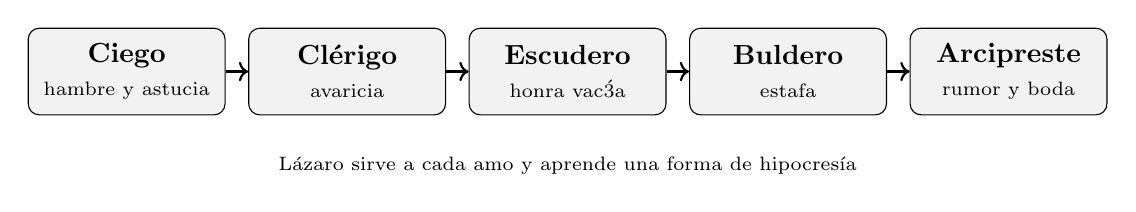
\begin{tikzpicture}
\tikzset{every node/.append style={align=center}}

\foreach \i/\x/\t/\u in {1/0/Ciego/hambre y astucia,2/2.8/Clérigo/avaricia,3/5.6/Escudero/honra vacía,4/8.4/Buldero/estafa,5/11.2/Arcipreste/rumor y boda} {
  \node[draw, rounded corners, fill=gray!10, minimum width=2.5cm, minimum height=1.1cm, align=center] (n\i) at (\x,0) {\textbf{\t}\\ \scriptsize \u};
}
\foreach \a/\b in {1/2,2/3,3/4,4/5} \draw[->, thick] (n\a) -- (n\b);
\node[font=\scriptsize] at (5.6,-1.2) {Lázaro sirve a cada amo y aprende una forma de hipocresía};

\end{tikzpicture}
\end{document}
